\documentclass[tikz,border=6pt]{standalone}
\usepackage{pgfplots}
\pgfplotsset{compat=1.18}
\begin{document}
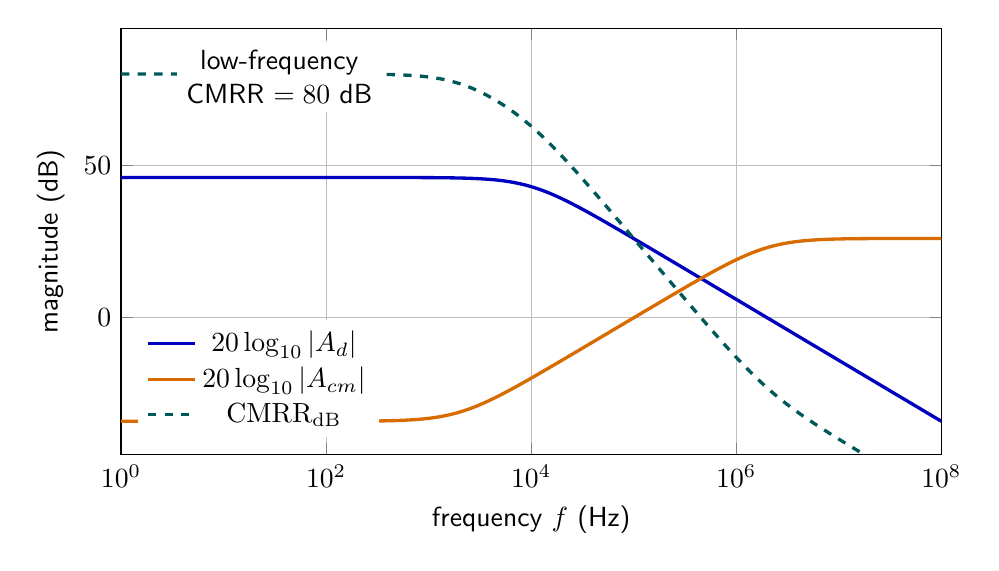
\begin{tikzpicture}[font=\sffamily]
\begin{semilogxaxis}[
 width=12cm,height=7cm,xlabel={frequency $f$ (Hz)},ylabel={magnitude (dB)},
 xmin=1,xmax=1e8,ymin=-45,ymax=95,grid=both,
 legend style={at={(.02,.04)},anchor=south west,draw=none,fill=white},
 xtick={1,1e2,1e4,1e6,1e8}]
 \addplot[blue!75!black,very thick,domain=1:1e8,samples=220]
 {20*log10(200/sqrt(1+(x/1e4)^2))};
 \addlegendentry{$20\log_{10}|A_d|$}
 \addplot[orange!85!black,very thick,domain=1:1e8,samples=220]
 {20*log10(0.02*sqrt(1+(x/2e3)^2)/sqrt(1+(x/2e6)^2))};
 \addlegendentry{$20\log_{10}|A_{cm}|$}
 \addplot[teal!70!black,very thick,dashed,domain=1:1e8,samples=220]
 {20*log10((200/sqrt(1+(x/1e4)^2))/(0.02*sqrt(1+(x/2e3)^2)/sqrt(1+(x/2e6)^2)))};
 \addlegendentry{$\mathrm{CMRR}_{\rm dB}$}
 \node[align=center,fill=white] at (axis cs:35,79) {low-frequency\\CMRR $=80$ dB};
\end{semilogxaxis}
\end{tikzpicture}
\end{document}
